\documentclass[a4paper,11pt,twoside]{report}
\usepackage[utf8]{inputenc}
\usepackage[top=2.5cm,bottom=2.5cm,outer=2.5cm,inner=2.0cm]{geometry}

\usepackage{amssymb}
\usepackage{amsmath}
\usepackage{booktabs}
\usepackage{hyperref}
\usepackage[noabbrev,capitalise]{cleveref}
\usepackage{colortbl}
\usepackage{color,soul}
\usepackage{xcolor}

\usepackage{enumitem}
% \setlist[enumerate,1]{label=\color{blue}(\arabic*)}
\setlist[enumerate,1]{label=(\arabic*)}

\usepackage{graphicx}
\usepackage{helvet}
\renewcommand{\familydefault}{\sfdefault}

\usepackage{hyperref}
\hypersetup{
	colorlinks = true,
	linkbordercolor = {white},
}

\usepackage{listings}

\usepackage{setspace}
\renewcommand{\baselinestretch}{1.3}

\usepackage{siunitx}
\usepackage{threeparttable}
\usepackage{multirow}
\usepackage{subcaption}


\begin{document}

\begin{center}
	{\large\textbf{Imaging Neuroscience \#203: Responses to Editors and Reviewers}}
\end{center}

% Robin: cortex / brain stem / hippocampus /

% ========================================
%     Editor
% ========================================


% ========================================
%     Reviewer 989
% ========================================

\noindent \underline{\textbf{Reviewer \#989}}

\textit{I thank the Authors for responding to all of my comments.}

\hspace{1em} {\color{blue} Thank you for your review.}

\vspace{1em}

\noindent \textit{Some minor points:}

\begin{enumerate}
    \item [1)] \textit{I think it would be good to have a mention in the Materials and Methods section of the replication that you put in the Supplementary Information to make readers aware it is there.}

    \hspace{1em} {\color{blue} Done.}

    \item [2)] \textit{Perhaps I missed it, but I did not see it stated whether the participant in the Supplementary Information gave informed consent. I would suggest adding a statement confirming informed consent was given in the Supplementary Information.}

    \hspace{1em} {\color{blue} Done.}

    \item [3)] \textit{Fig. 6: Description of what the arrows mean is missing from caption.}

    \hspace{1em} {\color{blue} Done.}

    \item [4)] \textit{pg. 30: "Alternatively, the multi-echo acquisition could be used..." should I think be "Alternatively, a multi-echo acquisition could be used..."}

    \hspace{1em} {\color{blue} Done.}

\end{enumerate}


% ========================================
%     Reviewer 990
% ========================================
\clearpage
\noindent \underline{\textbf{Reviewer \#990}}

\textit{Authors have partially addressed my previous comments. A list of pending issues is listed below:}

\vspace{1em}

\noindent \textit{\# Major:}

\vspace{1em}

\begin{enumerate}
    \item [3.b.1)] \textit{Sorry, still cannot see any particular limitation for applying denoising before shot combination in MUSE. Shot reconstructions for all diffusion measures from MUSE could be concatenated and PCA applied before multi-shot combination. I invite to consider testing this approach as well (if not appropriate, please provide reasons for not doing / state as future line).}

    \begin{figure}[h]
        \centering
        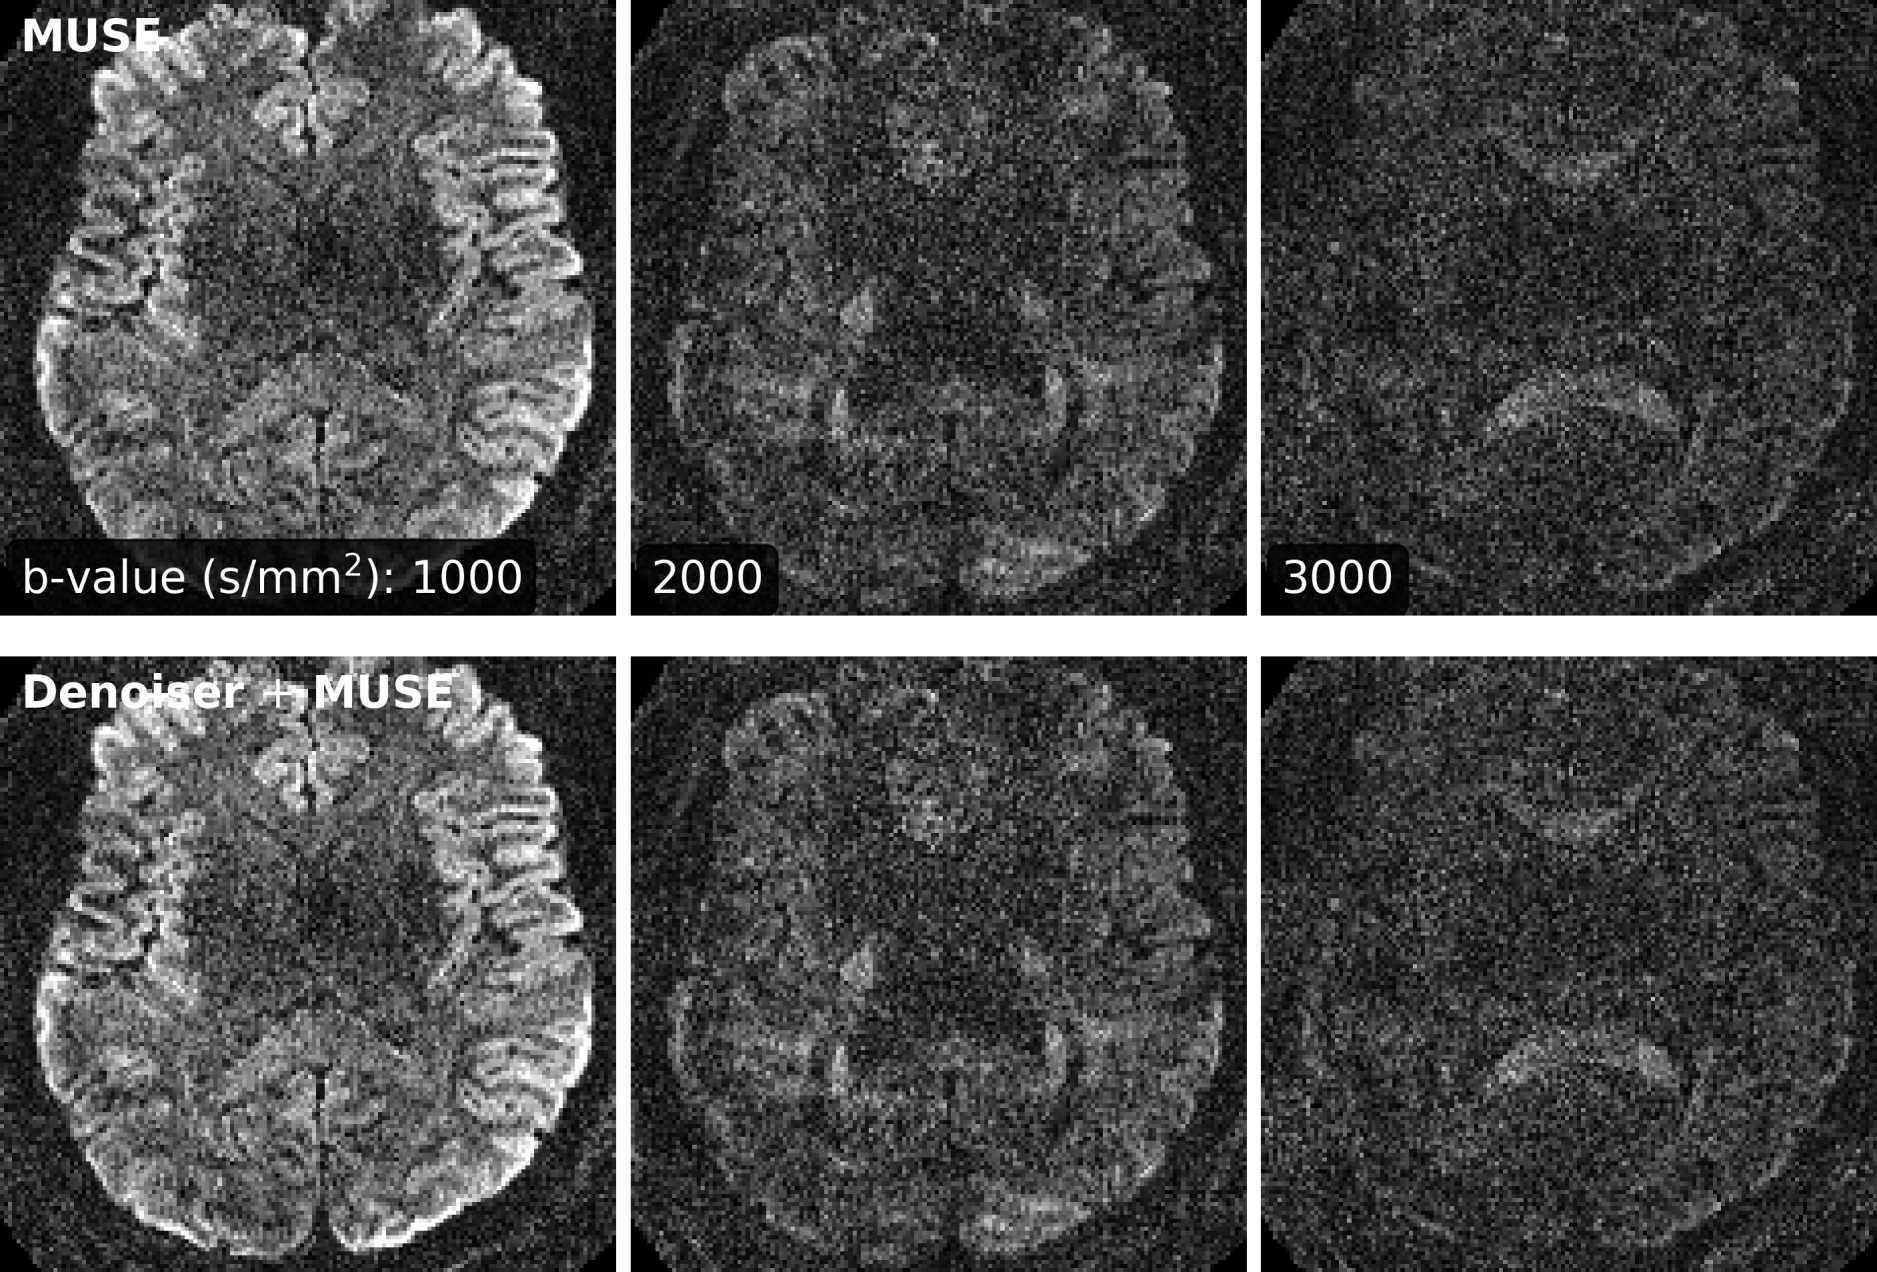
\includegraphics[width=0.8\textwidth]{denoiser_muse.png}
        \caption{Comparison of three-shell DWIs with data
        acquired by Protocol \#1 in Table 1.
        (Top) The standard MUSE reconstruction.
        (Bottom) The MUSE reconstruction with the local PCA denoiser
        applied before the multi-shot combination.}
        \label{FIG:DENOISER}
    \end{figure}

    \hspace{1em} {\color{blue} Thank you for the question.
    We applied the local PCA denoiser before multi-shot combination,
    and compared the results with the standard MUSE
    without PCA before multi-shot combination.
    The final reconstructed DWIs exhibit no major difference
    between these two approaches, as shown in \cref{FIG:DENOISER}.
    Shot images are reconstructed from the central $k$-space data,
    and thus have coarse resolution.
    As a result, the local PCA denoiser, when applied to the shot images,
    is less effective compared to its application to
    full-resolution shot-combined images.
    We included this result in both Figure 9 in the manuscript
    and Figure S5 in Supplementary Information.
    }

    \item [3.b.2)] \textit{Discussion on synergies between LLR and local PCA may be misleading. Authors mention that the "denoiser performs hard thresholding" but the cited approach is actually performing "singular value shrinkage", not thresholding (see first line of abstract). "use of LLR regularization for image reconstruction followed by the denoiser as a post-processing step" $\rightarrow$ but these are closely related methods based on similar principles, so why a substantial benefit to be expected in applying one on top of another?, why not fusing them trying to get the best of both? I think that discussion should focus on synergies rather than seeing them as separate steps.}

    \hspace{1em} {\color{blue} Thank you for the suggestion.
    We rewrote this paragraph and focused more on synergies.}

    \item [4.a)] \textit{I dont't think this is properly attended. In Fig.~6 you refer to block sizes of 3, 6 and 9, which is not matched to widths of 1, 2 and 4 as block size is square of width. Note 6 is also mentioned in text as baseline block size, which also seems erroneous. Also, in new text, "This observation agrees with the suggestion that the patch size should be no smaller than and close to the diffusion directions (Cordero-Grande et al., 2019)." But in (Cordero-Grande et al., 2019), patch sizes are automatically estimated. Have looked again for reported suggestion in the manuscript without success. Also, whilst patch sizes inducing close to square matrices could be intuitively better for large matrices, that's not so clear for small matrices as here (4 columns). Thus, usage of this motivating sentence seems rather speculative / forced, so sentence could be deleted or else further details should be provided. See also related minor point 9.}

    \hspace{1em} {\color{blue} Thank you for pointing this out.
    We delete the sentence in the manuscript.}

    \item [4.b)] \textit{L. 314 Please report meaning of "partially overlapping" (i.e., specific parameters of overlap) and also meaning of red arrows in Fig. 6.}

    \hspace{1em} {\color{blue} Done.}

    \item [7)] \textit{Please, explicitly include criteria for slice / diffusion encoding selection in the manuscript for Figs.~4-9 (including further clarifications to those provided in response for Figs.~7 and 9).}

    \hspace{1em} {\color{blue} Done.}

\end{enumerate}


\noindent \textit{\# Minor:}

\vspace{1em}

\begin{enumerate}
    \item [9)] \textit{I appreciate authors efforts to clarify this issue. Unfortunately, new results raise an important previously hidden issue. From Figure 1 in Responses to Editors and Reviewers, seems a normalization of singular values by block width would produce more comparable thresholds. This normalization is commonly used to counteract normalized eigenvectors with variable lengths. If agreed, experiments should be repeated by proper normalization of singular values, and modifications performed to methods presentation, including novel thresholds reporting. Please provide a detailed list of changes in your response. Otherwise, please explain why this normalization is not appropriate. This is related also to some of the concerns in major point 4, as, without proper normalization, optimal patch size is mainly driven by adequacy of preset threshold.}

    \hspace{1em} {\color{blue} Very good observation.
    Following your suggestion, we added the normalization option.
    As shown in \cref{FIG:NORMALIZATION}, the normalization
    (i.e., division of singular values by the corresponding block width)
    does normalize the largest eigenvalue,
    but shows small deviations in other eigenvalues.

    \begin{figure}
        \centering
        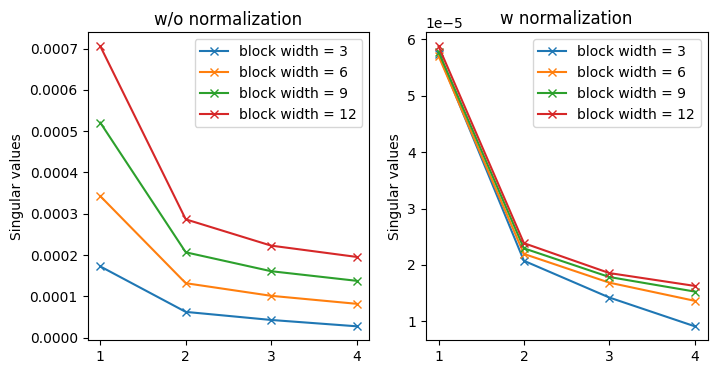
\includegraphics[width=0.8\textwidth]{normalization_llr.png}
        \caption{Comparison of singular values
        (left) without and (right) with normalization.}
        \label{FIG:NORMALIZATION}
    \end{figure}

    \hspace{1em} In the LLR denoising function,
    we first divide the singular values by the block width,
    perform singular value soft thresholding,
    and then multiply the thresholded singular values with the block width.
    As shown in \cref{FIG:NORMALIZATION_BRAIN},
    this normalization strategy does not render the same denoising effect
    for different block widths. This can be identified in the difference image
    from the block width of 9, which shows residual structural edges,
    whereas the diffrence image from the block width of 3 does not.
    Moreover, note that the soft thresholding is
    a nonlinear operator. Thus, the normalization strategy
    is not balanced and scales the thresholded singular values.

    \begin{figure}
        \centering
        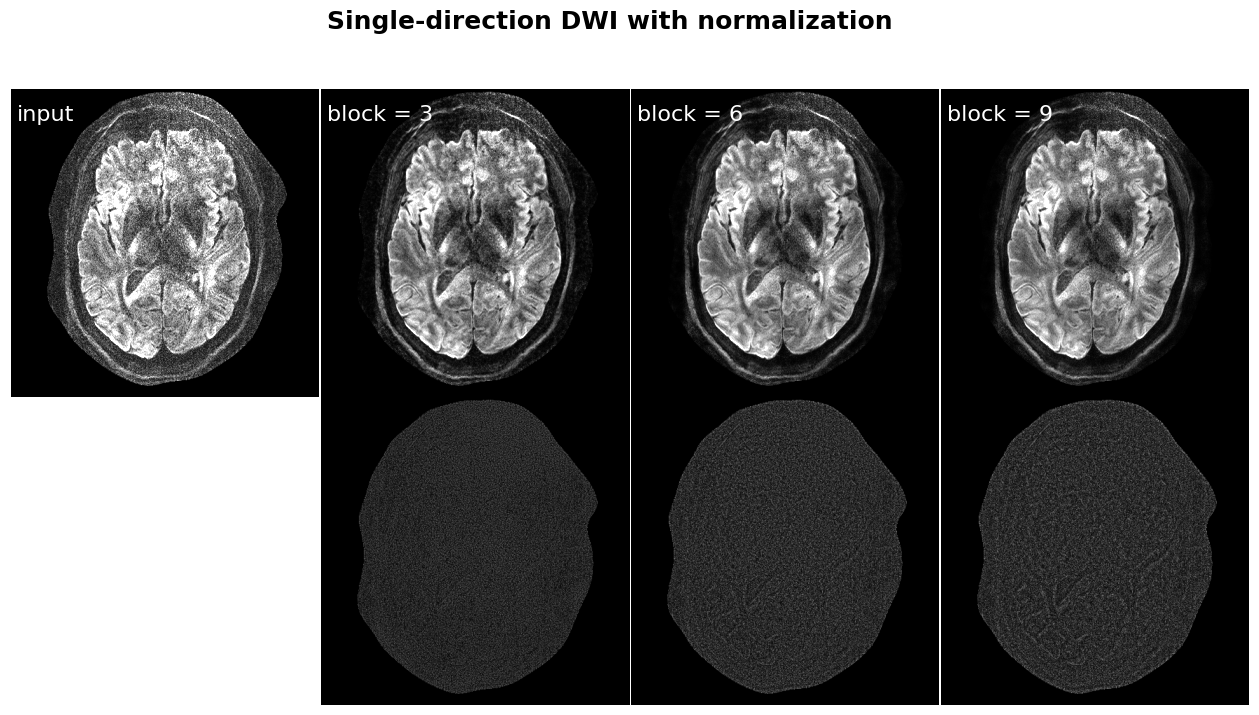
\includegraphics[width=0.8\textwidth]{normalization_1.png}
        \caption{LLR denoising with normalization. (Top) The first image shows the input to the denoiser.
        The other three images show the denoised output with different block widths. (Bottom) The difference between the input and the denoised outputs.}
        \label{FIG:NORMALIZATION_BRAIN}
    \end{figure}

    \hspace{1em} Please refer to
    \url{https://github.com/ZhengguoTan/demo_jets_diffusion_mri_7t/blob/main/demo_llr.ipynb}
    for the implementation and the interactive demo.
    }

    \item [12)] \textit{Thanks, unclear why this needs to be iterative rather than controlled by single filtering step parameters. Also, from eq.~6 you'd be smoothing the magnitude as well, not only the phase, so presentation of this equation may require modifications. Please, explain and report how you choose the number of iterations.}

    \hspace{1em} {\color{blue} Very good point, and thank you for the suggestion.
    First, we found out that the iterative procedure in Eq.~6,
    $\mathbf{x}^{(k+1)} = \mathbf{F}^{-1} \mathcal{H} \mathbf{F} \mathbf{x}^{(k)}$,
    is equivalent to setting a single filtering parameter,
    $\mathbf{x} = \mathbf{F}^{-1} \mathcal{H}^K \mathbf{F} \mathbf{x}$
    with $K$ the number of iterations.
    Second, as shown in \cref{FIG:FILTER_WIDTH,FIG:FILTERED_PHASE},
    the scalar exponent $K$ controls the width of the filter.
    A larger $K$ renders a narrower filter width.
    Consequently, the shot phases without filtering ($K = 0$)
    show ripple-like artifacts, whereas aggressive filtering (e.g., $K = 160$)
    removes shot-to-shot phase variation.
    Therefore, We chose $K = 5$ in this work.

    \begin{figure}
        \centering
        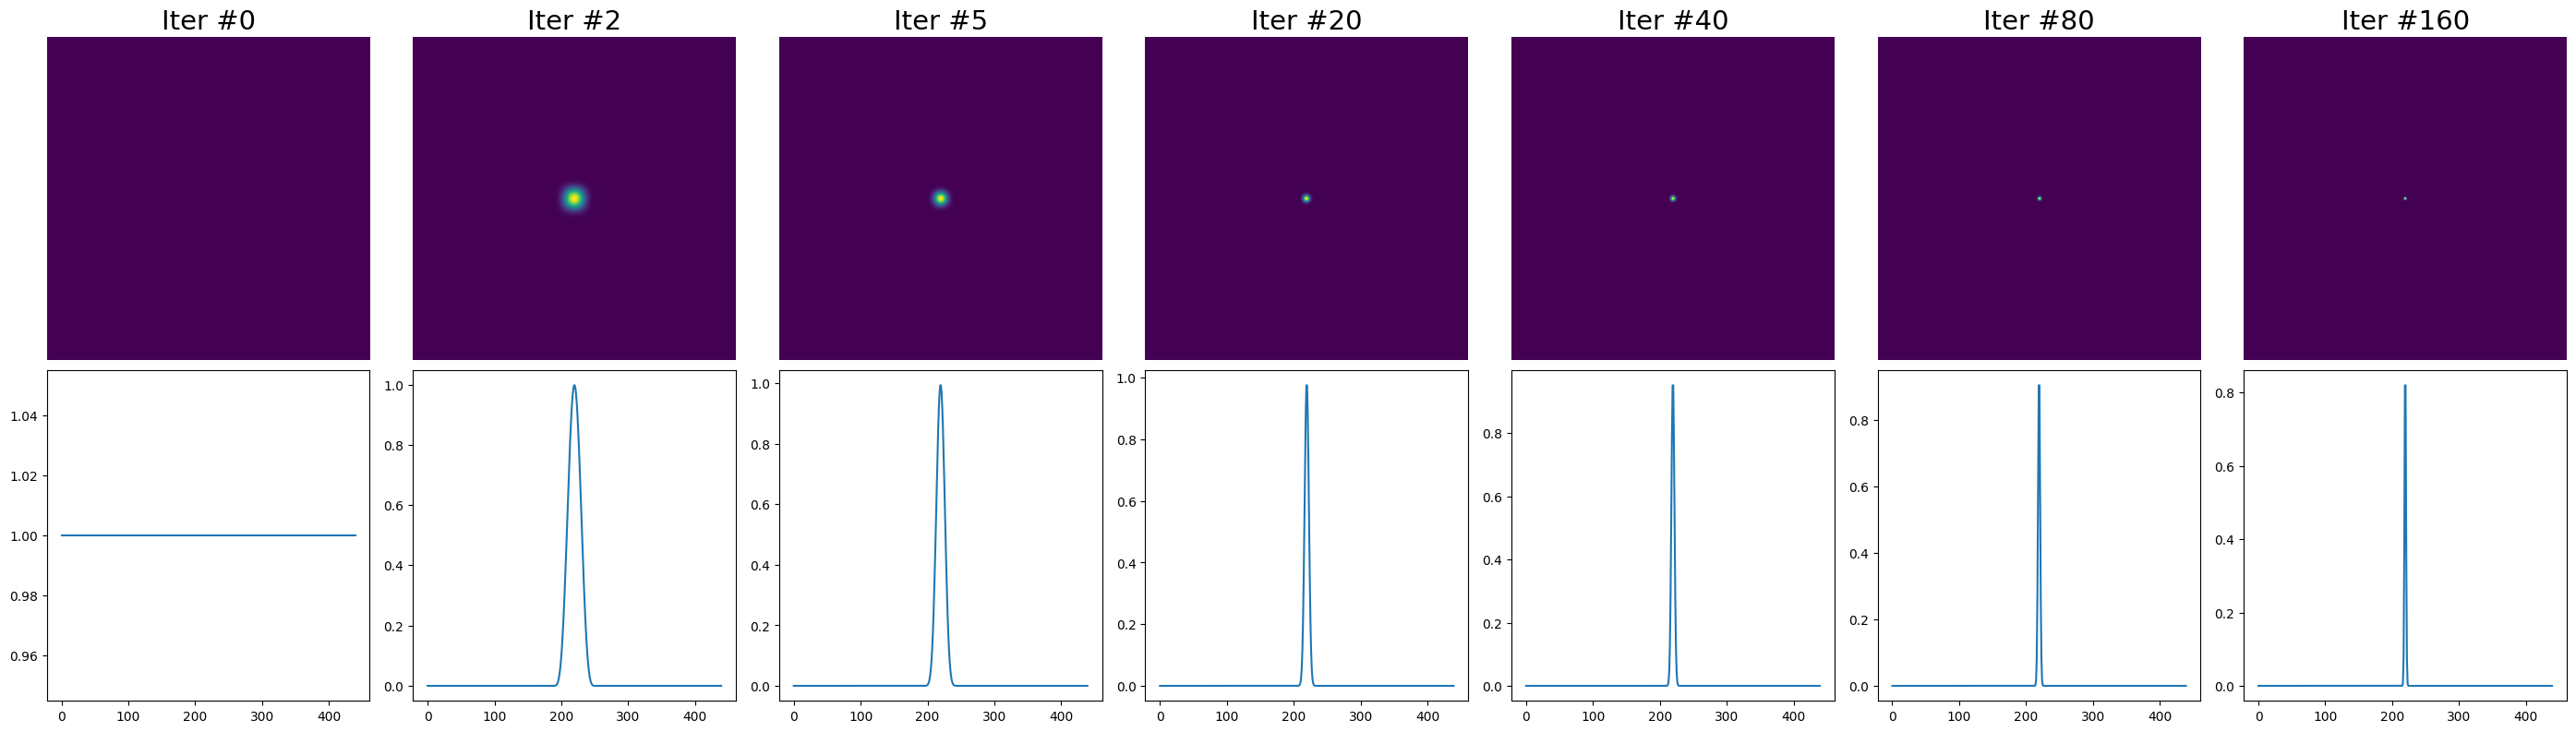
\includegraphics[width=\textwidth]{filter_width.png}
        \caption{(Top)Filters as a function of the iteration number $K$.
        (Bottom) Line profiles crossing the center of corresponding filters.}
        \label{FIG:FILTER_WIDTH}
    \end{figure}


    \begin{figure}
        \centering
        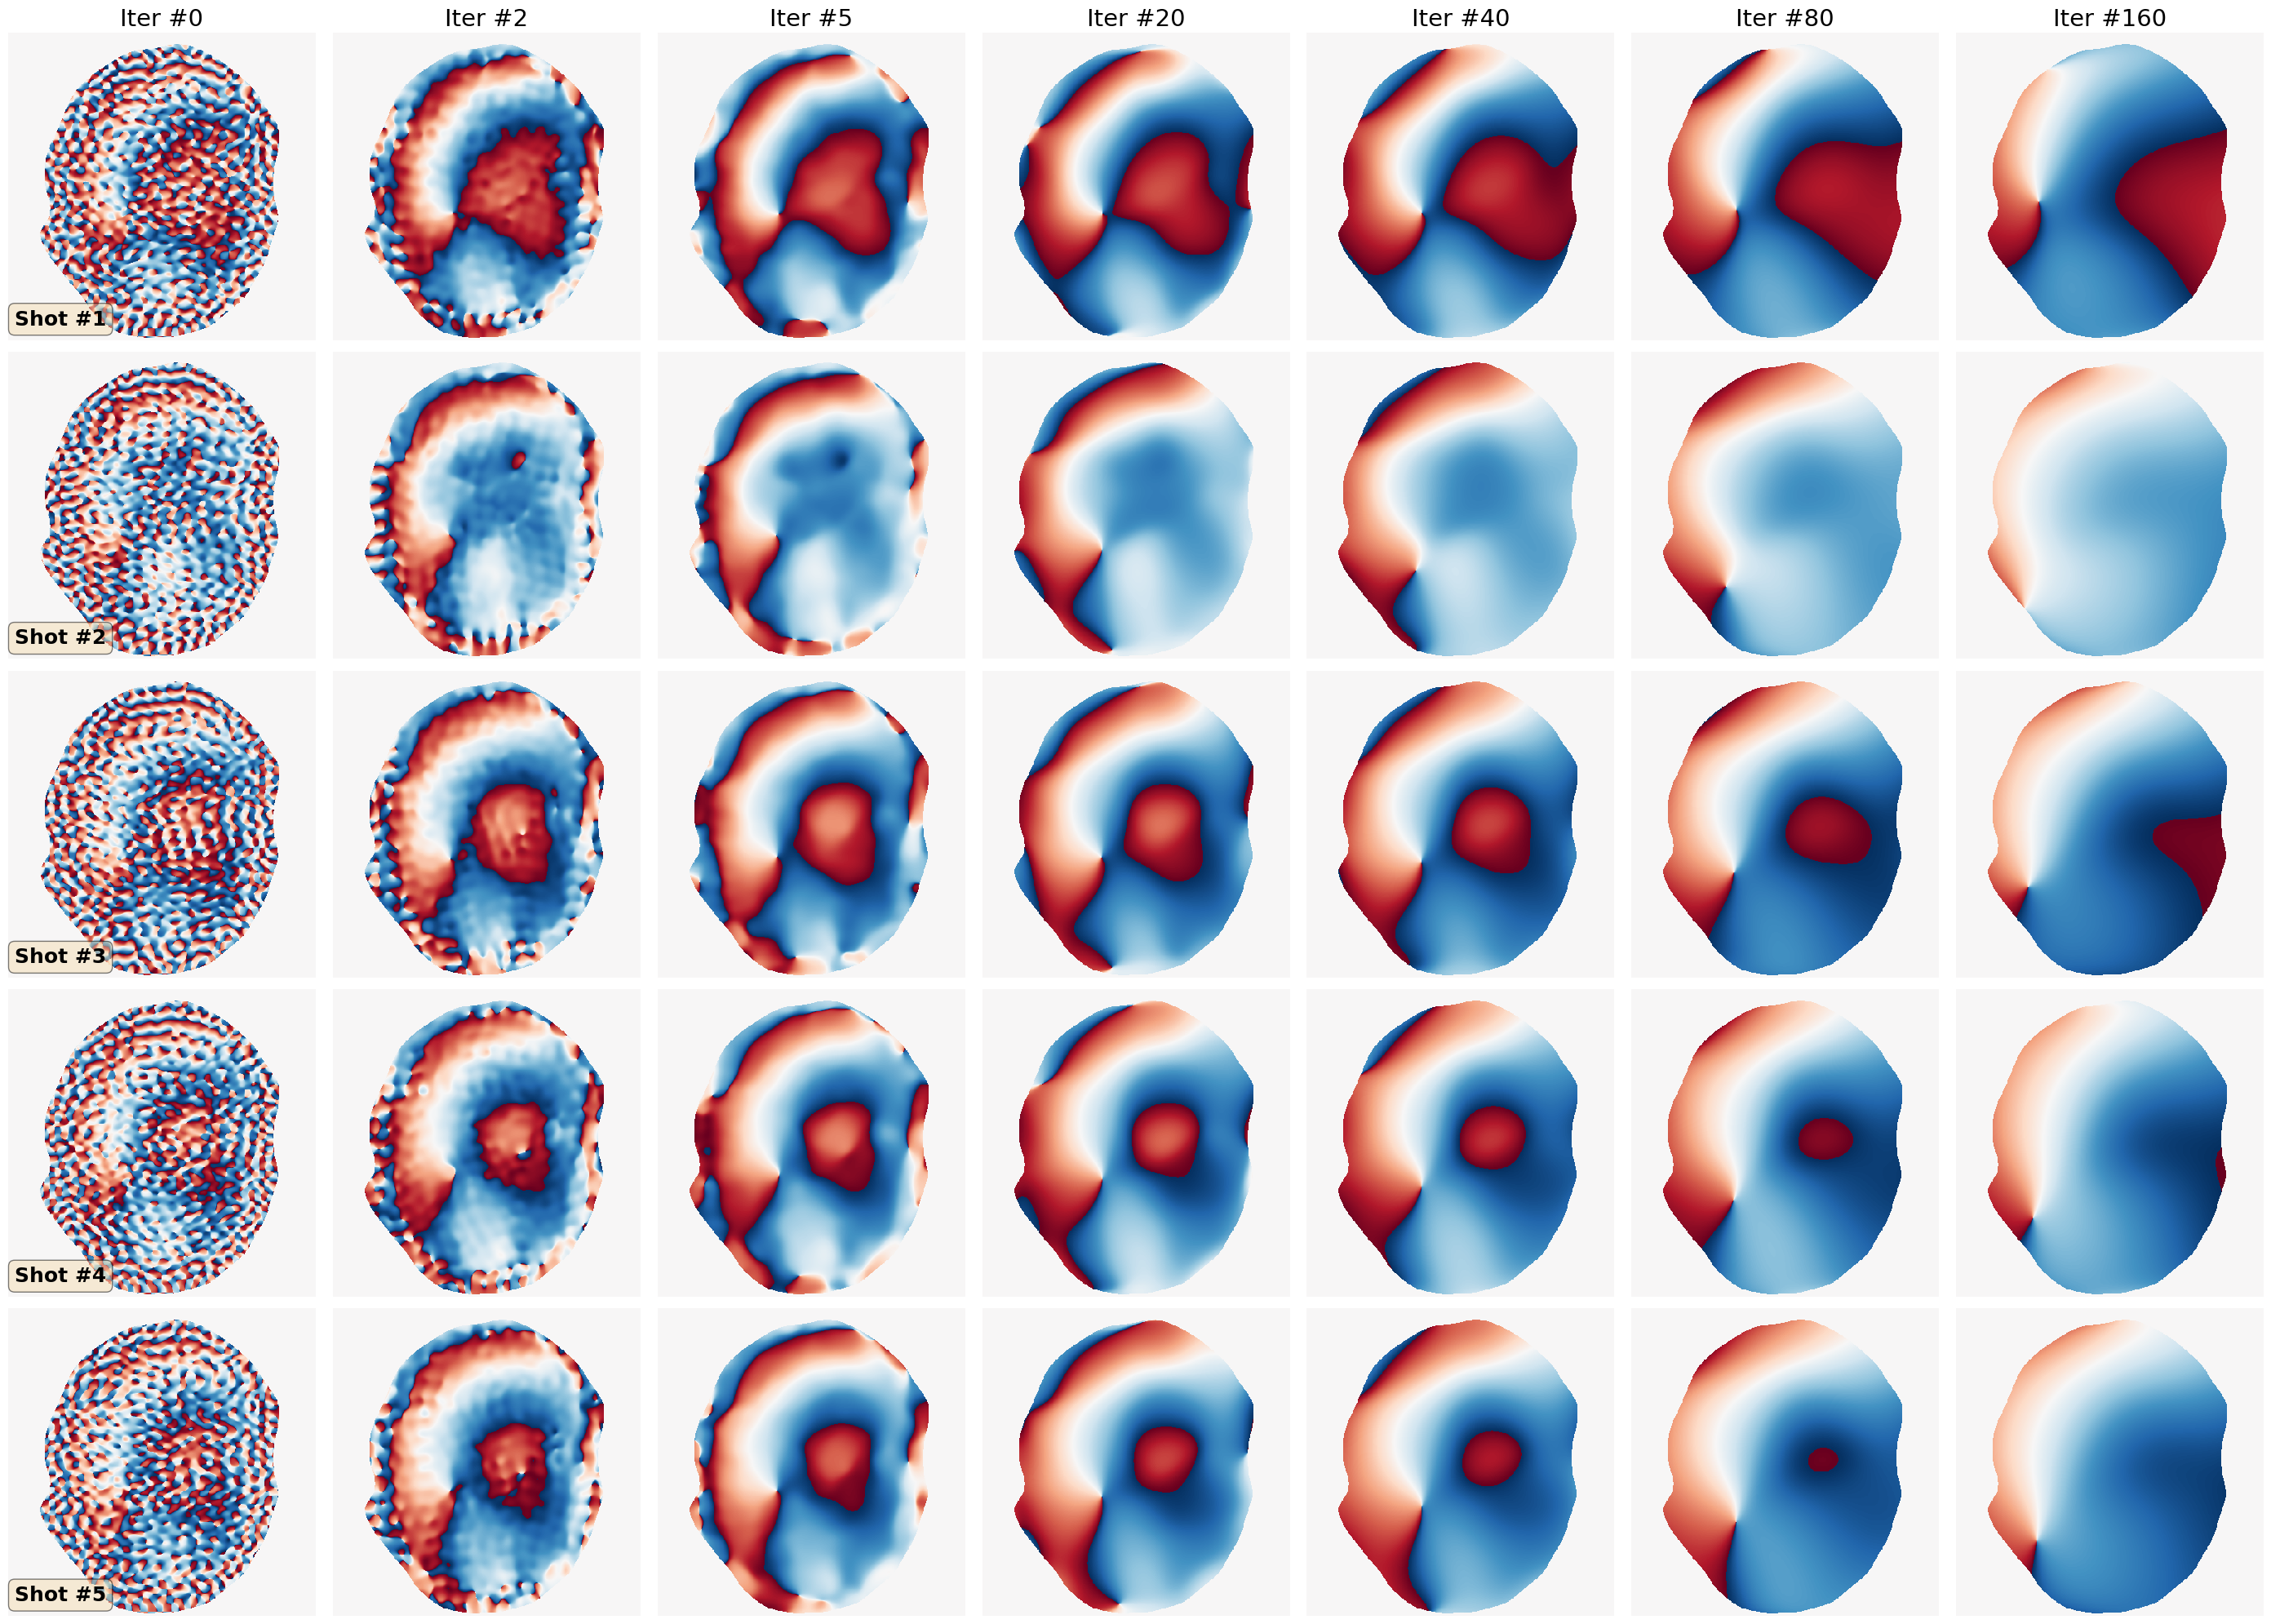
\includegraphics[width=\textwidth]{filtered_phase.png}
        \caption{Filtered shot phases with varying scalar exponents $K$.}
        \label{FIG:FILTERED_PHASE}
    \end{figure}

    }

    \item [13)] \textit{(New content) L369 "the multi-echo"  $\rightarrow$ "a multi-echo".}

    \hspace{1em} {\color{blue} Done.}

\end{enumerate}

\end{document}